\clearemptydoublepage
\chapter{Towards Enforcing Structural OCL Constraints using Constraint Programming}

\section{Introduction} 
\label{sec:intro}
% \ytodo{with \autoref{sec:motiv} 1 1/2 pages}
%\begin{outline}
% \1 OCL is the most common constraint language in MDE. 
% \1 While it is designed to verify constraints, several problems in MDE require from a way to enforce constraints: Model repairing \mtodo{cite}, model generation \mtodo{cite}, model completion \mtodo{cite}, design space exploration \mtodo{cite}
% \1 Existing work enforces OCL constraint by using Alloy, ... \mtodo{cite}. 
% % \mnote{some problems require arithmetic constraints that are not supported, efficiency for large models/search spaces, ...}{particularly important}
% \1 Reasons for CSP:
% \2 CSP provides access to optimised algorithms for Global Constraints.
% \2 Previous work results in applying Prolog Algorithm built on languages of $\rightarrow$ (and now arithmetic): Alloy. Which builds up a solution. Theoretically infinite but limited by memory.
% \2 Or Previous work only manages to apply CSP algorithms to attributes of the model. Which carves out a solution, which also means you must be able to see the sides, which means finite problems, taking into account the limited memory.

% \1 There is work on enforcing OCL constraints on integer attribute values, that are the most natural subject for CSP constraints. \mtodo{cite theo} 
% \1 In this paper we study how to apply CSP constraints to structural constraints, i.e. constraints that predicate on links among model elements
% % \1 The contributions are: 
% %    \2 a standard for identifying OCL to enforce with solvers
% %    \2 general solution for modeling queries involving variable references and/or attributes
% %    \2 The CSPs for the OCL Expressions here, and some constraints for some OCL words. 
%    \2 procedure to build these specific query CSPs
% \1 We evaluate the approach by measuring the size of CSPs

%\end{outline}
The Object Constraint Language 
(OCL)\footnote{\url{https://www.omg.org/spec/OCL/2.4/}} is a popular language in Model-Driven Engineering (MDE) to define constraints on models and metamodels. OCL invariants are commonly used to express and validate model correctness. For instance, logical solvers have been leveraged to validate UML models against OCL constraints, used by tools like Viatra \cite{Bergmann2015-viatra}, EMF2CSP \cite{Gonzalez2012-emf2csp} and Alloy~\cite{Jackson2002-alloy}.
% ,jackson_alcoa_2000
However several problems in MDE require a way to automatically enforce constraints on models that do not satisfy them, e.g. to complete such models or repair them.
% \ynote{This can also help implement proof assistants, such as Alloy \cite{jackson_alloy_2002, torlak_kodkod_2007} can find counter proofs to models and assertions upon them.}{too soon?}
% Other problems require to generate models from scratch, that satisfy a given set of constraints\mtodo{add citation Varro}.
Because of its combinatorial nature, the problem of enforcing constraints can be computationally hard even for small models. 

%Model Transformations \ytodo{\cite{}MT} come in flavours such as: model generation \ytodo{\cite{}}, model repair\ytodo{\cite{}}, view generation\ytodo{\cite{}James?}, model weaving \ytodo{\cite{}}, etc... Some of these problems require enforcing OCL constraints.
% \ytodo{more expressive languages encourage bigger problems.}
%These problems can be hard, which motivates us to find more efficient faster solutions.
%A particular transformation problem which interests us is that of Model Set Exploration \cite{schatz_design-space_2010, le_calvar_toward_2019}, which could be specified with a language using constraints.

% When solving such problems, there are two dominant strategies, which can be combined:
% building a solution (space) from inferences, and cutting down a space to carve out a solution.
% A popular technique is generate and test, which uses both heuristics, to in turn generate a solution (space) with positive inferences, and cut it down with negative inferences as counter arguments for potential solutions.
% This is the dominant strategy in related works such as 
% \mtodo{\ytodo{(Why CP) trying to very quickly give the intuition on why this work has an \emph{important difference}, and this is probably where we should start citing \emph{all} related work.
% Alloy \ytodo{\cite{}Alloy}, 
Constraint Programming (CP) aims to efficiently prune a solution space by providing tailored algorithms. Such algorithms are made available in constraint solvers like Choco \cite{Prudhomme2022-choco} 
in the form of global constraints. 
% propagation techniques to reduce the variable domains.
% , tailored to do so.
%As CP's focus is on reducing the search space, we will use an ATL \cite{jouault_transforming_2006} model transformation to first build a fixed solution space, Choco to find a solution within and OCL as bridge between modeling worlds.
% Hoping CP techniques can provide a boost in solving times.
Leveraging such global
constraints would potentially increase the performance of constraint enforcement on
models.
However, mapping OCL constraints to global constraints is not trivial. 
%While some OCL operations' semantics seem close to a global constraint, such as \texttt{isUnique} and \texttt{AllDifferent}, there is also the question of which variables the constraint is applied to, as a result from OCL's query language.
% One of the main problems is that most global constraints predicate on integers and booleans.
% While global constraints for graphs variables exist, the catalogue for such constraint is generally not very expressive or efficient.
Previous work 
% by Le Calvar et al. 
\cite{Le_Calvar2021-solvers} has started to bridge from arithmetic OCL constraints to arithmetic CP models, but it exclusively focused on constraints over attributes.%, found though \ynote{deterministic queries}{deterministic isn't the word} what we will later define as constant queries.

% We take the first steps to solving for all model properties.

%Similar work proposes solutions to this problem:
%SolverRational for QTV \cite{petter_solving_2009} which translates the transformation to prolog,
%CSP(M) for Viatra \cite{horvath_dynamic_2012,schurr_cspm_2009}, a solver developed for this specific purpose.

In this paper we focus instead on structural constraints, i.e. OCL constraints that predicate on the links between model elements.
%In other words, we want to model the problem of finding the variables upon which the operations will be enforced.
% We propose a first mapping for such constraints to global constraints in Choco.
% In this paper 
In detail, we present a method in two steps: 1) we provide an in-language solution for users to denote CP variables in OCL constraints; 2)  %a standard for identifying OCL to enforce with solvers, 
%the beginnings of a general solution for modeling queries involving variable references,
%and its addition to a previous implementation.
% we present our contributions. a standard for identifying OCL variables to give to solvers,
we describe a general CP pattern for enforcing annotated structural OCL constraints, i.e. constraints predicating on navigation chains. 
% , and the translation of several common OCL operations.
% 3) a strategy to refactor the OCL around the annotations.
To evaluate the effectiveness of the method, we discuss the size of the Constraint Satisfaction Problems (CSPs) it produces, and the resolution time in some examples.

The paper is structured as follows. In \autoref{sec:motiv} we present a problem on a UML model as our running case. In \autoref{sec:contrib} we describe how we annotate CP variables in OCL.  
In \autoref{sec:contrib2} we show how we model the annotated UML and OCL problem as a CSP.
% In \autoref{sec:contrib} we present our contributions. a standard for identifying OCL variables to give to solvers,
% a general solution for modeling queries involving variable references and/or attributes (in the context of references as sequences),
% some csps for some OCL keywords (in the context of references as sequences),
% and the procedure to build these specific query CSPs.
% In \autoref{sec:impl} we describe our implementation over the ATLc flavor of OCL.
In \autoref{sec:eval} we determine the size and performance of the resulting CP model.
In \autoref{sec:disc} we discuss limitations and future work.
In \autoref{sec:related} we look at related work.
Finally, we conclude in \autoref{sec:qed}.

% \section{Definitions/preliminaries}

% \begin{outline}
% \1 OMG/OOP vocab
%     \2 Modeling
%         \3 Object
%         \3 Properties
%     \2 Link <-> Reference
% \end{outline}

\section{Background and Running Case} \label{sec:motiv} 
% \ytodo{with \autoref{sec:intro} 1 1/2 pages}

% \begin{outline}
%     \1 Size of problem $10^{80}$
%         \2$\forall i \in Types : N_i$ number of Objects of Type $i$.
%         \2$\sum_{i,j\in Types | i \leq j}2^{N_iN_j}$
%         \2 $2^{O^2}$
% \end{outline}

For illustrative purposes, throughout the paper we exemplify the method on a well-known example, about Reconfigurable Manufacturing Systems (RMS). Notice however that the way to enforce constraints presented in this paper can be applied to any class diagram with OCL constraints. 

\subsection{Reconfigurable Manufacturing Systems}
% \ytodo{Explain UML and OCL without any notions of .var()}
An RMS \cite{Koren1999-rms} is an industrial solution to the problem of varying product demand.
In the most common version of the problem (from~\cite{Wang2012-srms}), a factory is organised into subsequent stages of identical machines.
To change the productivity of the factory, machines are added and removed from stages.
Manufacturing tasks are allocated to stages, and are generally at least partially ordered.
RMSs provide a number of problems to solve, such as:
matching tasks and machines with stages,
optimising those matches to achieve new productivity goals, 
as well as allocating the products to a machine of the stage it's going through,
or planning machine maintenance.

% \ttodo{these next sentences are very dry and disjoint}

% From this example we will take a structural constraint, to consider how to solve for it.
% % In this example we focus on the structural aspect of constraints of an RMS. 
% (constraints on attributes have already been studied in previous work \ynote{\cite{lecalvar_coupling_2021,le_calvar_toward_2019}}{I removed Petter from here, because they do it with logic}). 
% \ytodo{Theo: We focus our example on structural constraints that were not supported in our previous work. (was suggested before we realised it's double blind)}
% % Thus, we omit constraints that affect exclusively object attributes.
% In these examples, constraints are written with OCL queries which can be split in a variable and a constant parts.
% These constant parts are used as source for variable parts, when these variables affect references we call them variable references.

% These type of constraints use queries, which may present deterministic and variable portions, to find attributes and references upon which to to be applied.
% The variables and constraints of these problems pertain to OCL collections and their operations, in the specific case they represent References.
% The sources of the variable portion of queries are variable references, which are a particular case of OCL collections.

\begin{outline}
% \1 RMS
    % \2 what is reconfigurable manfacturing systems?
    % \2 \cite{wang_scalability_2012} example

% \1 UML model inspired from example
    % \2 changes are to illustrate contributions
        % \3 deeper navigation
    % \2 instance keeps the same task precedence tree and number of stages, gives a problem size

% \1 OCL Constraints(Expressions) inspired from example
    % \2 Same Characteristic Constraint
    % \2 Precedence Constraint
    % \2 Stage Size Constraint
    % \2 Budget Constraint
 
    % \2 cardinality constraints
    %     \3 a.b.c.size < 12
    %     \3 stage.tasks.size < 14
    %     \3 configuration.stages.tasks.size < 140
    %     \3 configuration.stages.machines.sum < 140 \ytodo{not a structural constraint}
    % \2 includes (making cycles/patterns)
    %     \3 a.var(c)->includesAll(a.var(b).var(c))
    %     \3 RMS Characteristic Constraint
    %     \3 stage.characteristics->IncludesAll(stage.var(tasks).characteristics)
    %         \4 this is like \cite{wang_scalability_2012}
    %         \4 but we could add more variables
% \1 general OCL problems
%     \2 Structural OCL Constraints
    % \2 mixing variable and deterministic navigation?
%     \2 Collection Constraints
\end{outline}


\subsubsection{A Class Diagram for RMS}
\begin{figure}[t]
\includegraphics[trim={0 0 0 0},scale=0.8]{Articles/SAC2025/figures/uc_uml.pdf}
\caption{Class Diagram for RMS Task constraints} \label{fig:uc_uml}
\Description[class diagram of RMS]{}
\end{figure}

\autoref{fig:uc_uml} uses a class diagram to describe the concepts of an RMS, and how they relate (inspired by~\cite{Wang2012-srms}). In this figure, we focus on the graph structure of the model (classes and references among them), omitting attributes. We use the class diagram flavor from the Eclipse Modeling Framework (EMF)\footnote{\url{https://eclipse.dev/modeling/emf/}}, that connects classes by unidirectional \emph{references}, instead of bidirectional \emph{associations}. 

% \footnote{In the use case we're taking inspiration from, all the machines had the same characteristics. We chose an arbitrary number of characteristics to illustrate possible sizes of the resulting CSPs.}
%From it we take 
%the number of stages and tasks to get information about problem sizes, 
%the task precedence tree,
%and an estimate number of machines.
% Larger than the number of stages, smaller than the number of machines.
% equal to the max cardinality of our problem. 
% \ttodo{last two sentences read weird ?}
% \ttodo{I don't understand last part of this sentence}
% Because of the constant nature of the relations linking tasks, machines and characteristics, the optimal implementation doesn't ask the CP solver to compute those matches. 
% In light of this, for our particular use case,  the number of characteristics doesn't have to effect the final size of the CSP. 
% \ttodo{werll, this could be rewritten in a simpler way}

The two main components of a reconfigurable manufacturing system are stages, and machines which are organised into stages.
% Stages have three properties of which two are attributes (stageId and maxMachines) and one is a containment reference to machines.
% Stages are totally ordered and have a numeric label to materialise it, the stageID.
% Common practice in RMS is to label them 10, 20, and so on.
% Thus we represent it as an attribute.
% Additionally, each stage has a maximum number of machines.
A \texttt{Machine}'s property is its relation to a set of \texttt{Characteristics}.
% and for each machine a cost attribute.
% All the machines of a stage must share the same characteristics.
Objects of type \texttt{Task} are partially ordered, as expressed by the \texttt{prev} reference.
%, this order introduces precedence constraints, not addressed here.
% modeled by the prev reference.
% Which  to our problem.
Tasks have two other properties: a reference to a \texttt{Stage} (allocating the task to that stage), and a reference to characteristics (i.e., the machine characteristics needed to perform the task). Similarly to the example in \cite{Wang2012-srms}, tasks and machines can be linked to any number of characteristics.

\subsubsection {OCL Constraints for RMS}

\begin{listing}
\begin{lstlisting}[language=ocl]
context Task inv SameCharacteristicConstraint: 
    self.stage.machines.forall(m | m.characteristics
        ->includesAll(self.characteristics)) 

context Task inv PrecedenceConstraint: 
    self.stage.stageNum >= self.prev.stage.stageNum
\end{lstlisting}
\caption{RMS Task constraints in OCL.} \label{lst:uc_ocl}
\end{listing}

The class diagram shown in \autoref{fig:uc_uml} cannot encode all constraints that are required for an instance to be a correct RMS instance.
%Some of the qualities of an RMS cannot be described with the pure UML Class Diagram of \autoref{fig:uc_uml}.
Additional constraints can be specified using OCL. 

\autoref{lst:uc_ocl} shows the two constraints we use as running example in this paper.
These are the structural constraints for tasks, part of a more detailed constraint model for RMS, with budget and productivity constraints.

OCL provides a way to query a model. 
For a given object, or collection of objects, we can query properties using "\texttt{.}", in expressions following an $objects.property$ pattern. 
Their properties can be references or attributes. 
In our running example, tasks have a reference to a stage, named \texttt{stage}, representing the stage a task is assigned to. In the OCL in \autoref{lst:uc_ocl} line 2, from the context of a \texttt{Task}, we query its \texttt{stage} by the expression \texttt{self.stage}.
The sub-expression \texttt{self} resolves to an individual object of type \texttt{Task}. 
The whole expression resolves to another object, of type \texttt{Stage}, associated with the task.
We can see this as a navigation starting at a \texttt{Task} node, and traversing the reference to the associated \texttt{Stage} node. We can chain navigations: e.g. to find the machines of the stage of a given task in \autoref{lst:uc_ocl} line 2 we use 
\texttt{self.stage.machines}.
% In this example we can see 
%OCL provides a language to query the model, and operations to apply on the results of the queries.
%In these constraints the \emph{top level} operations ($<$, $includesAll$, $forall$, $sum$,...) describe constraints on the queries \emph{below}.
%To navigate the model in a query, OCL uses navigation or attribute calls, which can be chained.
%In the OCL expressions of autoref{lst:uc ocl}, the operation is symbolised by ".", for example in $stage.machines$.
% \mtodo{This is ATLc flavor of OCL, give a short description}
% \ttodo{add line numbers from listing to each constraint paragraph?}
% \texttt{StageSizeConstraint} (\autoref{lst:uc_ocl}, \autoref{lst:ocl:var:size}) limits the number of machines that can be assigned to a stage.
% Because each stage can have a different value for $maxMachines$, this constraint cannot be represented using an upper bound on the cardinality of the machines reference.
% %In the class diagram we cant detail the cardinality for the individual stages, but that information is available as attribute of the stage object.
% %Thus we limit the size of the collection representing the links of the reference.

\texttt{SameCharacteristicConstraint} ensures that \emph{the machines of the stage performing a task} have all the required characteristics. From the given task (\texttt{self}) we navigate to the stage where it is performed, and find all the machines of that stage (\texttt{self.stage.machines}). For each machine \texttt{m} we impose that the set of \texttt{characteristics} it supports  (\texttt{m.characteristics}) includes all the characteristics required by the given task (\texttt{self.characteristics}).

\texttt{PrecedenceConstraint} ensures that tasks with precedence are performed after their predecessors, i.e. they are assigned to the same stage or a later one.\footnote{The constraint uses the \texttt{stageNum} constant integer attribute that indicates the position of the stage in the manufacturing line, omitted in \autoref{fig:uc_uml}.}
%\footnote{In our model for brevity, the order of the pointer variable domains corresponds to the order of stages in the instance. In the more detailed model, a constant attribute of \texttt{Stage}: \texttt{stageID} represents the order among stages.\mtodo{I would prefer to add stageID to the metamodel and constraint, or just remove PrecedenceConstraint, that is never used}}
% \mtodo{add explaination for readers that do not know OCL}

We will consider these constraints in the following three scenarios.
\begin{description}
    \item[S1:] machines have already been assigned to stages, and the assignment of tasks to stages must be found;
    \item[S2:] tasks have already been assigned to stages, and the assignment of machines to stages needs to be found;
    \item[S3:] both tasks and machines must be assigned to stages.
\end{description}
%To identify these different scenarios
% , possibly with additional information to model the problem.
%we propose annotations in the OCL, described in \autoref{ssec:varop}.
% \ynote{
% In the larger scope of our work, the OCL is written as part of an ATL transformation, and work under the assumption a variety of transformations can/will be applied to a model.
% % In the context of model exploration, we often have to find new information, such as the position of an object instance in a graphical user interface resulting from a transformation.
% }{maybe move to discussions}

% for the task to be performed.
% The third constraint describes the relation between a task and the machines of the stage it's associated to.
% All the machines of the stage associated to a task must fit the task's characteristics requirements.

% \texttt{BudgetConstraint} (\autoref{lst:uc_ocl}, \autoref{lst:ocl:var:budget}) describes a budget constraint stating that the total cost of machines of all the stages stays below a given threshold.%, an arithmetic constraint on the sum cost of the used machines.
% % \ttodo{\ytodo{Because budgets are sometimes exceeded, in the implementation we will introduce constraint relaxation here}}

% Overall, the constraints in  \autoref{lst:uc_ocl} focus on the association of tasks and machines with stages. Enforcing these constraints may alter the structure of the model graph, this is why we speak of structural constraints.
% %In order to complete the description, \autoref{lst:uc_ocl} uses the object constraint language.

% \subsection{Example of RMS Object Diagram}
% \begin{figure}
% \includegraphics[width=\linewidth,trim={0 0 0 0}]{figures/uc_instance.pdf}
% \caption{Example of RMS model.} \label{fig:uc_uml_instance}
% \end{figure}
% % \begin{figure}
% % \includegraphics[trim={0 0 0 0},scale=0.5]{figures/RMSinstanceexampleoptimum.pdf}
% % \caption{RMS Use Case instance optimum} \label{fig:uc_uml_instance_optimum}
% % \end{figure}
% % \ytodo{name tasks and characteristics, put one solution, two solutions? to show variability}
% \autoref{fig:uc_uml_instance} shows a small instance which conforms to the class diagram in \autoref{fig:uc_uml}. 

% Continuous lines represent the initial model (i.e., the initial state of the factory), that does not satisfy the constraints (\autoref{lst:uc_ocl} $+$ multiplicity constraints). 
% We have 4 tasks, 3 machines and 2 stages.
% The three first tasks involve drilling air holes and an attachment point for a bolt, which could be performed by a drill or a mill,
% % , requiring a drill.
% while the last task (tapping) requires a tapping machine.
% % Task precedence is shown in the diagram with the arrows.
% The arrows between tasks express the precedence relations.

% We want to automatically enforce the constraints, to compute a new correct state for the factory. A possible solution we may obtain is represented in \autoref{fig:uc_uml_instance} by considering both continuous and dotted lines.  
% In particular dotted lines represent the references introduced after automatically enforcing the constraints. 
% % but before that there's a choice of machines for the drilling.
% % \ytodo{Make link variables doted}
% All stages have been linked to tasks and machines, while respecting the constraints of task precedence, characteristics compatibility, maximum stage size and budget.
% %These links are unknown,
% % from the instances of our use cases, 
% %and this is the information we want to find with CP, while conforming to \autoref{fig:uc_uml} and \autoref{lst:uc_ocl}.
% % And in the future optimise them.

%\subsection{Model Navigation in OCL}

% \ytodo{We can also see this a finding "where we are" in a graph, and moving from nodes to nodes}

%\mdelete{The previous query can be seen as the prior sub-query to this one.
%Finding those machines is trivial when the associations between objects are known, which is the normal process when validating a model. 
%But when enforcing constraints, such as searching for a model, the question of which machines this expression resolves to has to be solved.
%This syntax for model navigation isn't part of standard Constraint Satisfaction Problems.
%However it can be systematically modeled using global constraints as we will show in this paper.}

% \subsubsection{Size of the Search Space}
% Because in our scenarios we want to complete a model instance, such that it conforms to the OCL constraints, a primary question is the complexity of the problem.

% % \ynote{
% % To understand the size of the space, we'll use our Use-Case to fix the size of most of the dimensions. 
% % }{weird}
% Taking inspiration from \cite{wang_scalability_2012} for the aspect of our model, we also get information about the number of objects in the problem instance. 
% In our running example, our instance will have 4 stages (S) and 43 task (T), directly taken from \cite{wang_scalability_2012}. We infer 24 machines (M) from their constraint model.
% For Characteristics little information was given, however, we consider all links to these objects as known data in all our scenarios. 
% % In some cases it will be used as a variable C.

% With a generate and test strategy, randomly associating tasks to a stage, and machines to a stage, and checking for solutions, there would be at most $S^{T+M}$ tests, in other words there are around $2.10^{40}$ possible graphs.

\subsection{Constraint Programming} \label{ssec: csp_intro}
% \stodo{
% TODO: Introduce the CP modelling, global constraints, why GC ? 
% }
%\stodo{\ytodo{check it out}}
CP is a powerful paradigm to model and solve combinatorial problems. In CP, a model, also referred as a CSP, is stated by means of {\it variables} that range over their {\it domain} of possible values, and {\it constraints} on these variables. A constraint restricts the space of possible variable values. For
example, if $x$ and $y$ are variables which both range over the domain $\{1, 2, 3\}$, the constraint $x + y \leq 4$ forbids the instantiations $(x, y) = (3, 2), (2, 3), (3, 3)$. While there are many types of constraints, the {\it global constraints} are perhaps the most significant - being the most well-studied - and have the ability to encode in a compact way combinatorial substructures. A global constraint is defined as a constraint that captures a relation between a non-fixed number of variables.

%Constraint Satisfaction Problems gives us another declarative modeling paradigm.
% not too dissimilar to MDE.
%Constraint programming allows us to build CSP instances and find solutions to them.

%CSP declarations are composed of variables, their domains, and constraints linking them.

%Constraints can be arithmetic: $x < 4$, logical: $x \rightarrow y$, but additionally Global Constraints exist.
%Global constraints are sometimes the result of efficient algorithms for solving general puzzles (which can model problems) or combinations of constraints, or generalizations of other constraints, for example. 

The $allDifferent$ constraint is probably the best-known, most studied global constraint in constraint programming. It states that all variables listed in the constraint must be pairwise different. For instance the Sudoku problem can be naturally modeled with $allDifferent$: fill a $n \times n$ grid with digits so that each column, each row, and each block contains all of the digits that must be different. 
%In Sudoku the rules state numbers must be different, or $\neq$.
%But specifically all the numbers of a row, column, or area, must respectively be \emph{allDifferent}, or $allDifferent$.
%All Different is a global constraint, which neatly models problems such as Sudoku
%\footnote{the CP aspect of sudoku with alldiff is providing the constraints with the right variables, which is a fixed problem for sudoku, but not in our use case because of the nature of the query language provided by OCL}, but also offers improved solving over a clique of $\neq$ constraints.
% Using arithmetic constraints, logical constraints, and a selection of global constraints, we are able to programmatically build the CSP corresponding to our running example.
% % Two non-trivial constraints used here are the element constraint, and global cardinality constraint.
% A non trivial constraint used here is the element constraint.

In this paper we will specifically make use of the \emph{element} constraint.
% \noindent {\bf The Element Constraint} 
%\subsubsection{The Element Constraint}
% The Element Constraint.
Let $y$ be an integer variable, $z$ a variable with finite domain, and $vars$ an array of variables, i.e., $vars = [x_1, x_2, \ldots, x_n]$. The element constraint $element(y,vars,z)$ states that $z$ is equal to the $y$-th variable in $vars$, or $z = vars[y]$. The element constraint can be applied to model many practical problems, especially when we want to model variable subscripts.

\subsubsection{Propagation}
%Here we can look at both propagation, and how the element constraint passes information between our variables.
Propagation for a constraint is the action of updating the domains of the variables bound by that constraint.
When solving, propagations will generally run when the domain of one of the variables bound by the constraint is updated.
% , propagating the information across the model.

For instance, let $y=\{0,1\},x_0=\{0\},x_1=\{2,5\}, z=\{-10..10\}$ be the domains of the variables given to the element constraint.
% (\mnote{z has all possible integer values}{in the previous section it's written that z must have finite domain}). 
The element constraint's propagator can update the domain of $z$ to $\{0,2,5\}$.
The meaning of this propagation is, the possible values for $z$ are a subset of the union of possibilities for $x_y$, here the union of $x_0$ and $x_1$.
If during another constraint's propagation, or during search, 0 is removed from the domain of $z$, such that $z=\{2,5\}$, the element constraint can update the domain of $y$ to just $\{1\}$.
Here, because the domains of $x_0$ and $z$ are disjoint, then $z$ can not be equal to $x_0$, hence the element constraint propagation can remove 0 from the domain of $y$.
%From here-on we have $y=1,z=x_1$.
Finally, if the element constraint is given the following variable instances: $y=0, x_0=0, z=2$, propagation for the constraint would tell us it is not satisfiable, and serve as a counter proof in model validation.

Propagation is one of the fundamental pillars of constraint programming, along with modeling and search.
Global constraints spanning a large number of variables allows one to leverage propagation to the fullest.
The application of propagation to the problem of OCL is our fundamental difference to much of the related work.
To apply it to OCL we need a systematic way to model OCL expressions using gobal constraints, and particularly to model OCL query expressions.

\section{Denoting CP Variables in OCL Expressions}\label{sec:contrib}\label{ssec:varop}

In this section we describe the first step of the methodology we propose, i.e. a method to select what parts of UML and OCL to model in CP.
In a second step, described in Section~\ref{sec:contrib2}, the resulting annotated OCL will be translated to a CP model. 
%how to model what one could see as the core of OCL expressions and especially 
%how to model OCL expressions including structural constraints; %, i.e. \texttt{NavigationOrAttributeCallExp}; 
%3)
% Which we may call \texttt{PropertyCallExp} or property access for brevity.
%how to refactor OCL expressions, to make the CSP smaller and faster to solve.

% \ynote{Our first contribution, the annotation of OCL, allows us to split the task of resolving OCL keywords between standard OCL engines, and CSP solvers.}{
% What we have is a way to split an OCL expression between a part that can be interpreted like normal OCL and a part that must be enforced by a constraint solver.
% }

% The second contribution,
% \ynote{Theo: we have a generic CSP encoding for navigation across variable references in OCL expression}{
% is a CSP model for the OCL AST Object \texttt{NavigationOrAttributeCallExp}, which is prevalent across OCL problems, as it provides the core of OCL model querying, and directly impact the size of all CSPs - modeling OCL expressions - using integers as we do.}

% \ynote{And third, with solving complexity in mind, we provide a method for rewriting OCL expressions with properties annotated as variable. To derive information before building the CSP, resulting in smaller search spaces.}{
% I'd say we have a way to rewrite some OCL expressions to make them easier to solve
% }



% In the problems described with the UML of \autoref{fig:uc_uml} and \autoref{lst:uc_ocl_var}, our variables are the references from task to stage, and from stage to machines.

% In this paper the variables represent the relations between objects.

\begin{listing}
% (*@\label{lst:ocl:var:prev}@*) context Task inv PrecedenceConstraint:
%     self.var('stage') >= self.prev.var('stage')
    \begin{lstlisting}[language=ocl, numbers=none]
-- Scenario S1
(*@\label{lst:ocl:var:char:s}@*) context Task inv SameCharacteristicConstraint:
    self.var('stage').machines
        ->forall(m | m.characteristics
            ->includesAll(self.characteristics))
-- Scenario S2
(*@\label{lst:ocl:var:char:m}@*) context Task inv SameCharacteristicConstraint:
    self.stage.var('machines')
        ->forall(m | m.characteristics
            ->includesAll(self.characteristics))
-- Scenario S3
(*@\label{lst:ocl:var:char:sm}@*) context Task inv SameCharacteristicConstraint:
    self.var('stage').var('machines')
        ->forall(m | m.characteristics
            ->includesAll(self.characteristics)) 
\end{lstlisting}
% --     self.stages.machines->sum(m | m.cost).weak("<", self.budget.value)
% (* context Object def: 
%     var(property: String) =
%     self.eGet(property) *)
\caption{Denoting variables in \texttt{SameCharacteristicConstraint} from \autoref{lst:uc_ocl} using \texttt{.var()} in accordance with the three scenarios.} \label{lst:uc_ocl_var}
\end{listing}

Since OCL was not originally designed for enforcing constraints, it does not include primitives to drive the search for a solution that satisfies the constraints, as typical CP languages do. 
For instance, it does not include a way to define which properties of the model have to be considered as constants or variables, while trying to enforce the constraint. 
Distinguishing variables from constants has a double importance, both for correctly modeling the CP problem, and for reducing its search space to a limited number of variables. 

Note that the distinction of variables from constants can not be performed automatically in general, as it depends on the user intent. 
% \ynote{
% For instance, given a model with too many machines for a stage, to enforce the \texttt{StageSizeConstraint} the user may want to: 1) consider the list of machines for a stage (\texttt{self.machines}) as a constant and increase the variable \texttt{maxMachines}, or 2) consider \texttt{maxMachines} as a constant and remove some machines from the variable \texttt{self.machines}. 
% }{
For instance, in our use-case scenarios, we want to enforce the reference between \texttt{Task} and \texttt{Stage} to conform to \texttt{SameCharacteristicConstraint} of \autoref{lst:uc_ocl}.
To do so we annotate the references for which information is missing, but for uses such as model repair, annotations can direct where to look for fixes in the model.
For instance given a factory configuration which breaks \texttt{SameCharacteristicConstraint}, we could choose between fixes reassigning tasks, or reassigning machines, or both to stages.
% }

To allow users to explicitly denote properties (attributes or references) in an OCL expression as variables (variable attributes or variable references), we propose the \texttt{var()} operator with the following syntax:
$$\texttt{source.var('property')}$$ where \texttt{source} identifies the objects resulting from the
prior sub-expression,
\texttt{property} is the name of one of the attributes or references of the objects. 
% and \texttt{flag} is an optional argument used to specify the encoding of variables. %for which parameters might required additional arguments.
% The required and first argument is always the property of the source class to be added to the problem.
% Additional arguments can be used to choose the encoding of the variable.
In \autoref{lst:uc_ocl_var} we apply the operator to \texttt{SameCharacteristicConstraint} in \autoref{lst:uc_ocl} for each one of our three scenarios, defining the properties that we consider as variables for that scenario. All properties that are not included in a \texttt{var()} operation call are considered constant.

% \ynote{Notice that we do not extend the OCL syntax, but we design the syntax for \texttt{var()} as a normal OCL operation, included in a specific library. On one side this allows us to reuse existing tooling for OCL with no adaptation. On the other side, while checking the constraint, we consider \texttt{var()} simply as a reflective navigation of the specified \texttt{property} (similarly to \texttt{refGetValue} in ATL/OCL\footnote{\url{https://wiki.eclipse.org/ATL/User\_Guide\_-\_The\_ATL\_Language\#OclAny_operations}}). Hence, for an OCL checker, the constraints in \autoref{lst:uc_ocl_var} are equivalent to the constraints in \autoref{lst:uc_ocl}.
% }{
Notice that our in-language solution does not extend the syntax of the OCL language, but we add an operation to the OCL library: \texttt{var(propertyName: string) : OclAny}. 
When the OCL constraint is simply checked over a given model (and not enforced), the \texttt{var} operation simply returns the value of the named property (as a reflective navigation).\footnote{Look at getRefValue from ATL/OCL for a similar reflective operation \url{https://wiki.eclipse.org/ATL/User\_Guide\_-\_The\_ATL\_Language\#OclAny_operations}}
Whereas, if one wants to enforce OCL, \texttt{var} is used as a hint to build the corresponding CSP.
% }

We can add extra parameters to \texttt{var} to drive CP modeling, e.g. for bounding the domain for a property, or choosing a specific CSP encoding among the ones presented in the next section. In future work we plan to add other parameters to guide model repair, by describing how much we can change properties in order to fix the model.
% \ynote{In our metamodel to-many cardinalities are unbounded, but an upper-bound is required for our model (based on Adjacency lists) to be finite. For example, if we want to bound the number of links between stages and machines to N' with such an annotation, we'd write to the effect of:
% }{when you talk about bounds, you could explain that we need to bound the cardinality of relations because CSP requires users to define all variables before solving and because it helps. I find this § a bit strange and out of order because you talk about adjacency list which is a detail of the encoding that you did not present yet. Maybe this part could be ignored for now and brought back when you present the encoding (and I'm still not a huge fan of this notation)
% }
% $$\texttt{stage.var('machines', 'AdjList', N')}$$

Note that, alternatively, users can also annotate the variable references in the metamodel, instead of the constraints. In this case, we can always statically translate such variable annotations on metamodels into the variable annotations on constraints discussed here.

%As we usually choose the variables when writing the constraints, we opted for the annotation proposed here. 

\subsection{Annotation in the OCL Abstract Syntax Tree}
The annotated OCL is parsed in the form of an AST. Given an instance model to solve for, each object will have their own instance of the AST, where \texttt{self} resolves to said object. \autoref{fig:uc_ocl_var_ast} shows the AST of \texttt{SameCharacteristicConstraint} from \autoref{lst:uc_ocl_var} Scenario S3. We show \texttt{var} annotations as dotted rectangles. 

\begin{figure}[ht]
    \centering
    \includegraphics[width=0.8\linewidth]{Articles/SAC2025/figures/ASTbasic.pdf}
    \caption{AST of \texttt{SameCharacteristicConstraint} from \autoref{lst:uc_ocl_var} Scenario S1, S2 \& S3.}
    \label{fig:uc_ocl_var_ast}
    \Description[AST]{}
\end{figure}

\autoref{fig:uc_ocl_var_ast} illustrates a key function of \texttt{var} annotations: they define the scope of the CP problem, i.e. a frontier between what can be simply evaluated by a standard OCL evaluator, and what needs to be translated and solved by CP. In \autoref{fig:uc_ocl_var_ast}, the scope defined by each \texttt{var} annotation is indicated by a dotted rounded rectangle. The \texttt{var} annotation requires everything \emph{inside} the corresponding scope to be translated to CP. 
 
For instance, since the reference between \texttt{Task} and \texttt{Stage} is annotated (\texttt{self.var('stage')}), the result 
% (meaning or location depending on your intuition) 
of the \texttt{stage} \texttt{NavigationOrAttributeCallExp} needs to be found by the solver.
% Therefore 
All nodes in the scope of an annotated node will be in the CSP, 
% \ynote{
as what they resolve to depends on the solution the solver is searching for.
% }{did I turn this into a riddle again?}
Conversely, nodes that are not in the scope of any \texttt{var} annotation do not need to be translated to CP, making the CP problem smaller.

The processing of the AST in \autoref{fig:uc_ocl_var_ast} (corresponding to Scenario S3) starts from the bottom: \texttt{self} is directly evaluated by standard OCL, as is \texttt{self.characteristics}.
However we don't know the result of \texttt{self.stage}, which implies we don't know the result of \texttt{self.stage.machines}.
% , even if from the context of a stage we may know \texttt{self.machines}.
Above, we iterate on the unknown machines and for all of them: ask what their characteristics are, and if they include the characteristics of the task.
% Essentially, 
All these questions must also be answered by the solver, which means
% To relate back to \autoref{fig:uc_ocl_var_ast}
any node of the tree within the dotted box must be resolved by the solver. 

In Scenario S2, \texttt{SameCharacteristicConstraint} from \autoref{lst:uc_ocl_var} has the same AST as in \autoref{fig:uc_ocl_var_ast}, but only the \texttt{machines} node is annotated as \texttt{var}. Hence, in this case the CP scope is smaller, since \texttt{self.stage} can be directly evaluated by OCL. 

% \ynote{
%All nodes above and including the lowest annotated as variable are in the box.
% }{well in your figure the two node on the right are above annoted nodes and are not inside CSP}
%The case of the \texttt{Task} to \texttt{Stage} reference being annotated as variable correspond to the larger box, while if only the reference from \texttt{Stage} to \texttt{Machine} is annotated, the solver deals with the smaller box.
% Annotated \texttt{NavigationOrAttributeCallExp} also draw the border between the OCL engine and the CSP solver domains quite clearly.
%The less nodes which must be resolved the smaller the CSP.

%The most common keyword we can see here, and in many OCL expressions, is the \texttt{NavigationOrAttributeCallExp}.
%It is the core of OCL's model navigation and property access, and the core of what we call queries and structural constraints.
%It also has a large impact on the size of the problem.
% If a task is possibly linked to $n$ stages, and those stages are each linked to $n'$ possible machines. 
% There are ${S \choose n} * {M \choose n'}$ possible links from tasks to machines though stages.
% Adding on top a query for characteristics, means ${S \choose n} * {M \choose n'} * {C \choose n"}$ possible query results.


% Given two types of object $obj_A$, $obj_B$, and two properties: a reference from objects of type $obj_A$, $reference2B$, and a property of objects of type $obj_B$ $Bproperty$, we can make the following query:

% $obj_A.reference2B.Bproperty$.

% Alloy $\rightarrow$ Bool $\rightarrow$ SAT

% us $\rightarrow$ Integers $\rightarrow$ propagation

\subsection{Refactoring OCL Around Annotations}
\label{ssec:refactor}

Given that everything above an annotated node of the AST is within the scope of the CSP, it's interesting to find strategies to reduce the scope as much as possible, as it results in a smaller CSP to solve.
The annotated expressions of \autoref{lst:uc_ocl_var}, all have their annotations low in the tree \autoref{fig:uc_ocl_var_ast}.
Ideally, all the annotations should be at the top of the tree.
% Having cut the OCL into constant and variable sub-expressions, and modeled the query problem in CSP, we can try to rewrite the OCL to generate the simplest CSP.
The semantics of the expression gives clues to refactor them, the expression requires that:
\emph{All the machines connected to a task (via a stage), each individually match the task's characteristics}
this is the same as requiring that:
\emph{The set of machines that match the task, includes the set of machines connected to the task}.

\begin{listing}[!t]
\begin{lstlisting}[language=ocl,numbers=none]
-- Scenario S1
(*@\label{lst:ocl:var:derive:s}@*) context Task inv SameCharacteristicConstraint: 
    inv: Stage.AllInstances()
        ->select(s| 
            s.machines.forall(c | c.characteristics
                ->includesAll(self.characteristics))
        ->includesAll(self.var(stage)))
-- Scenario S2
(*@\label{lst:ocl:var:derive:m}@*) context Task inv SameCharacteristicConstraint: 
    inv: Machine.AllInstances()
        ->select(m| m.characteristics
            ->includesAll(self.characteristics)
        ->includesAll(self.stage.var(machines)))
-- Scenario S3
(*@\label{lst:ocl:var:derive:sm}@*) context Task inv SameCharacteristicConstraint: 
    inv: Machine.AllInstances()
        ->select(m| m.characteristics
            ->includesAll(self.characteristics)
        ->includesAll(self.var(stage).var(machines)))
\end{lstlisting}
\caption{Annotated \texttt{SameCharacteristicConstraint} from \autoref{lst:uc_ocl_var} refactored around the annotations.} \label{lst:uc_ocl_derive}
\end{listing}

In \autoref{lst:uc_ocl_derive} we can see the result of this rewrite for all three scenarios.
The beginning of the expressions are now constant queries, and search for all the suitable machines (or stages), here isolated as \texttt{sel}: 
% $$\texttt{Class->AllInstances().select(...)}.$$
$$\texttt{let sel = Class->AllInstances().select(...) in}$$
At the end of the expression we state that selection must include the result of the variable query over the machines and/or stage of the task: 
% $$\texttt{select(...)->includesAll(...)}$$
$$\texttt{sel->includesAll(...)}$$

% A CSP Model for the semantics of \emph{forall} with incoming AdjLink Variables is trivial.
% $$(pointer_i \neq null) \rightarrow body(pointer_i)$$ where $body$ is the body of the forall applied to all the non null $pointer_i$ of the \texttt{AdjList}.
% If all the CSP resulting from the compilation of OCL can handle null pointers as input, this model isn't even necessary, and it simply directs compilation.

% It is possible to model \texttt{Forall} as part of a CSP based on \autoref{csp:nav}

% However, in the case where the body isn't a variable expression, we can derive information ahead of solving (propagation and search). 
% Because for a set of objects to satisfy an expression, that set of objects must be sub-set of the set of objects that satisfy the expression.
% And we can determine ahead of solving the set of objects that satisfy the constant expression.
% The outline of the strategy is to, forall objects of the source type (result of the variable expression), find if they satisfy the constant expression.
% We then constraint the result of the variable query to be among the conforming objects.

% This refactoring can be done systematically in OCL, as seen in \autoref{lst:uc_ocl_derive}, after which the compiler runs its normal course.

In \autoref{fig:uc_ocl_derive_ast} we can see the AST resulting from the parsing of the expression of \autoref{lst:uc_ocl_derive} Scenarios 2 and 3.
% \footnote{
%More accurately, this AST results from the annotation of \texttt{machines} (\autoref{lst:ocl:var:derive:m}), or the annotation of \texttt{stage} and \texttt{machines} (\autoref{lst:ocl:var:derive:sm}).
% When \texttt{stage} alone is annotated, the result of the machine navigation is added to the derived possibilities, which means the solver only resolves the inclusion directly on the problem variables.
% }
The AST is significantly different to the previous one, but most importantly, the number of nodes within the scope of the solver is greatly reduced, to just navigation and the top level constraint.
\begin{figure}[ht]
    \centering
    \includegraphics[width=\linewidth]{Articles/SAC2025/figures/ASTderive.pdf}
    \caption{AST of SameCharacterticConstraint from \autoref{lst:uc_ocl_derive} Scenario S2 \& S3}
    \label{fig:uc_ocl_derive_ast}
    \Description[AST]{}
\end{figure}
% \ytodo{This was originally done by hand with knowledge of the context, it seems generalisable but that's my next paper, please please accept this one so I can move on with my life}
% \ynote{
% This can be generalised to any constant expression, not just those body of a forall.
% It requires a new OCL operation (implementable in OCL): \texttt{PowerSet()}.
% Which simply takes the place of \texttt{AllInstances()}.
% This might also find use in building a portfolio of models to further leverage parallelised solving tools. 
% }{rewrite}
The CSP now only models the inclusion.%, and only requires a single instance of \autoref{csp:nav} for each task, when both \texttt{stage} and \texttt{machines} are annotated.
% One could also initialise the variables with the selected domains to the same effect.
% Said domain of possible values is the result of the \texttt{select(...)}.

We applied this strategy manually with knowledge of the context, but it is generalisable.
In the case of any constant sub-expression applied to a variable query, it is possible to determine candidates, or candidate sets, for that sub-expression and enforce the result of the variable query to be among them.
For example, for:
\texttt{self.var(ref).attrib<3}
we can find candidates which satisfy the constant sub-expression \texttt{.attrib<3}.
This adds more computation ahead of building the CSP, but also allows us to leverage the OCL engine in cases where it's more efficient such as this one.
% \noindent \texttt{context Task}

% \noindent \texttt{task.stage.machines.characteristics.includesAll(task.characteristics)}

% \smallskip \smallskip
% \noindent \texttt{context Task:compatMachines : Machine}

% \noindent \texttt{derive: Machines.AllInstances()->select(m | m.characteristics->includesAll(self.characteristics))}

% \smallskip
% \noindent \texttt{context Task}

% \noindent \texttt{inv: self.compatMachines->includesAll(self.stage.machines)}

% \section{Implementation}

% \begin{listing}
% \begin{lstlisting}[language=java]
% IntVar[] navCSP(IntVar[] source, IntVar[][] property, IntVar dummy){
% int n = source.length;
% int nn = property[0].length;
% int nnn = n*nn;
% IntVar[] out = m.intVarArray(nnn,MIN_VALUE,MAX_VALUE);

% IntVar[] dummies = new IntVar[nn]; 
% for(int i=0;i<nn;i++) dummies[i] = dummy;
% if(dummy.getValue()==0) 
%     IntVar[] table = concat(dummies,flatten(property));
% else 
%     IntVar[] table = concat(flatten(property),dummies); 

% int k=0;
% for(int i=0; i<n;i++) for(int j=0;j<nn;j++){
%     IntVar pointer = source[i].mul(nn).add(j).intVar();
%     m.element(out[k++], table, pointer).post();
% }

% return out;}
% \end{lstlisting}
% \caption{navCSP implementation using Choco Solver}
% \label{lst:navchoco}
% \end{listing}


\section{Modeling Annotated OCL Constraints using Constraint Programming}
\label{sec:contrib2}

To enforce OCL constraints on existing model instances using CP, we must encode parts of the model instances as CSP variables and constraints (\autoref{subsec:assoc}), and then encode the OCL using additional CSPs on the variables of the model instances (\autoref{subsec:expr}). 

\subsection{References in CP}
\label{subsec:assoc}

There are two main families of CSP, those using booleans, and those using integers.
Both of these can be used to model our problem.
In this paper we are focusing on structural constraints, which implies modeling references, and chains of references in OCL queries.
Simply put: using boolean variables we can ask whether two objects are connected, using integers we can ask how many times two objects are connected, but more interestingly: to which object a given object is connected to.
This last encoding uses variables as pointers, and is the one we will be presenting here.

% \noindent \textbf{Model} a model. Something that has properties and represents a system under study.
% A CSP is a model of which there are 2 kinds of properties: variables and constraints.

\noindent \textbf{Reference:} exists between two Classes;
can be seen as the lines in a class diagram such as \autoref{fig:uc_uml}.
An example from our use-case, is the references between \texttt{Task} and \texttt{Stage}.
Here our references are only navigable one way.
% , the direction of which is given named association end.
% These associations can be annotated as variable.
For an object diagram or an instance, reference instances are called \textbf{links}.
%\noindent \textbf{Reference} or association end,
%is where we find the name and cardinality of our associations.
%For example, in our use-case: objects of type \texttt{Task} each have a to-one reference to the class \texttt{Stage} named \texttt{stage}, and
%objects of type \texttt{Stage} each have a to-many reference to the class \texttt{Machines} named \texttt{machines}.
% Two references can be opposite ends of an association, but not seen in this paper.
References in an EMF instance, are instantiated as objects of the type EReference.

\noindent \textbf{Variable Reference:}
these imply adding variables and possibly constraints to the UML CSP.
% These may also be referred to as the problem variables in the context of our CSPs.
Non-annotated references will be called constant.
From annotation of the OCL we infer which references are variable.
From the expression \texttt{self.var(stage).var(machines)}, we can determine that for \texttt{Task} the reference \texttt{stage} is variable, and for \texttt{Stage} the reference \texttt{machines} is variable.
This is the bridge between the model instance and the CSP, when we find a structure in the CSP, we will update these references.

% \noindent \textbf{Occurrence Variable} boolean or integer.
% Respectively answers the questions \emph{are two given objects connected?} and \emph{How many times are two given objects connected?}
% The domain of integer occurrence variables is defined by the cardinality of the reference.
% An example variable of this type could be named $task_{21}stage_{2}$, if instantiated to $false$ or 0 meaning task 21 isn't connected to stage 2.

% \noindent \textbf{AdjMtrx Variable} models a variable reference instance in CSP. 
% List of occurrence variables between a given object and objects of the referred class.
% % Essentially the row of the adjacency matrix relevant to the given object.
% In our implementations each object has it's  

% \ytodo{commented occ, add figure for occ and ptr maybe}

\noindent \textbf{Pointer Variable:} integer variable answering the question \emph{which object is a given object connected to?}
The number of instances of the target class gives the upper bound of the variable's domain.
The lower bound being 0, in our model meaning \emph{null pointer}.
This happens when an object has less links than the maximum allowed by the metamodel or the annotation.

\noindent \textbf{AdjList Variable:} models a variable reference instance in the UML CSP.
Essentially an adjacency list,
it is a list of pointer variables associated with an EReference.
The number of pointer variables in an \texttt{AdjList} is defined by the cardinality of the reference, or can be informed by the annotations.
This choice is one of the main dimensions of the complexity of the resulting problem. 
These will be our primary \emph{problem variables}, as opposed to the intermediate variables the OCL expressions may require.
% We call an individual integer variable identifying an object a \emph{pointer} variable, a collection of which represents a reference as an Adjacency List, which we call here \texttt{AdjList} Variable.
% \texttt{AdjList} Variables, allow for additional information on the structure of a graph: links can be ordered and repeated, and their count can be detached from the count of objects.
% When adding an \texttt{AdjList} Variable to the CSP, we can choose the number of pointer variables to create. 
% \ynote{
% The choice can be informed by the cardinalities found in the metamodel, or additional annotations directing the modeling.  
% \ynote{
% During evaluation we will several choices for number of pointer variables, each will be identified as $N,N',N"$ or $N_{refID}$.
% }{
% Gotta clean this up
% }

% Similarly we name integer variables counting the connections between two objects, \emph{count} variable, a collection of which represents a reference as a row of the Adjacency Matrix, which we call AdjMtrx Variable. If two objects can only be connected once through a specific reference, boolean variables can be used.

\noindent \textbf{UML CSP:} what we call the CSP of the annotated instance properties.
It includes the above models of variable references, and any constraints the metamodel (\autoref{fig:uc_uml}) may define upon them, such as containment, uniqueness, coherence between opposite references, etc..
For our running example, the UML CSP only holds the problem variables, no additional constraints are applied because of the metamodel.
Regardless we're calling it a CSP because it is in the general case.

For our use case, the references from \texttt{Task} to \texttt{Stage}, and from \texttt{Stage} to \texttt{Machines} can be variable.
This implies for objects such as tasks, and specifically their reference to a stage, associating them to an \texttt{AdjList} identifying the stage with a single pointer variable.
Equally for stage objects, we associate their reference object to an \texttt{AdjList}, but with multiple pointer variables.
These all can be organised into tables, where for each object and a property, we match that property with CSP variables.
The row numbers of these tables are the actual domains of pointer variables. 
% In this paper we will be focusing on integers variables representing pointers to objects, and using off-the-shelf solvers to find conforming models.

\subsection{OCL Expressions in CP}
\label{subsec:expr}
With annotated references, navigation and querying become part of the CSP.
Given an OCL query expression such as \texttt{self.var(stage).machines}, if the CSP must determine which \texttt{Stage} is associated to a \texttt{Task}, it will also determine the set of \texttt{Machine} associated to the \texttt{Task} through the \texttt{Stage}.

% \ynote{
% \noindent \textbf{Variable Expression} Any OCL (sub-)expression for which the source is annotated. Any non-annotated OCL (sub-)expression will be called \textbf{Constant Expression}.
% For example from \texttt{self.ref0.var(ref1).attrib <3}, we have the variable expression \texttt{.var(ref).attrib < 3}, and the constant expression \texttt{self.ref0}.
% We can also isolate \texttt{.attrib <3} as a constant expression.
% }{
% feel like there might be some "flou" in there.
% After talking with Theo: maybe talk about variable navigations instead
% }
\noindent \textbf{OCL CSP:} 
Nodes within the scope of the solver are associated with a CSP, all of which combined make up the OCL CSP.
The models for the OCL expressions are built on top of the UML CSP, by reusing the problem variables modeling the instance properties.
% For example in: \texttt{self.var(attrib)<3}, the variables of \texttt{self.var(attrib)} are found in the UML CSP.
% The OCL CSP for the object instance would apply the \texttt{<3} constraint.
% Another example, \texttt{self.var(ref).attrib<3}, \texttt{self.var(ref)} are again UML CSP variables. 
The OCL node CSPs will generally also add their own intermediate variables to pass information upwards.
Constants of the model will also sometimes appear in the OCL CSP as integer variables, but their 
% domains constrained or initialised with the model data. 
% Their 
domain of possible values is $the$ value found in the model.


\noindent \textbf{Variable Expression:} if an OCL expression has an annotation, it is referred to as variable. If it has none we call it constant. Expressions can be decomposed into sub-expressions, and variable expressions can be decomposed into variable and constant sub-expressions.
A particular type of expression is the query, which in this paper are the primary sub-expressions of structural constraints.

% \noindent \textbf{Variable Query:} The sub-expression of a query for which the source is annotated or a variable query.  
% Non-annotated OCL (sub-)queries will be referred to as Constant.
% For example, in the precedence constraint from \autoref{lst:uc_ocl_var} \autoref{lst:ocl:var:prev}, we have two variable queries as branches of the structural constraint: \texttt{self.var('stage')} and \texttt{self.prev.var('stage')}, the latter has a constant sub-query \texttt{self.prev} as source to the variable sub-query.
% \ytodo{Variable Property Access vs Variable Navigation}

\noindent \textbf{Variable Query:}
variable queries are similarly any annotated query expression, but can be divided into two main parts: 
\begin{enumerate}
    \item \emph{variable property access}: \texttt{src.var(prop)} 
    \item \emph{variable navigation}: \texttt{.var(src).prop}.
\end{enumerate}
Variable property access is sourced from constant (non annotated) queries, e.g. \texttt{self.prev.var(stage)}.
Variable navigation is sourced from a variable query. 
For example in: \texttt{self.var(stage).var(machines).characteristics} machines and characteristics are reached through variable navigations, the first being from \texttt{Stage} to \texttt{Machines}, the second from \texttt{Machines} to \texttt{Characteristics} .

% \ynote{
% \noindent For example from \texttt{self.ref0.var(ref1).attrib<3}, we have the variable query \texttt{.var(ref).attrib}, and the constant query \texttt{self.ref0} as it's source.
% This query is the left branch of constraint expression \texttt{query<3} .
% }{adapt to above rewrite}

% \ytodo{So reading through what I wrote, I talk of UML and OCL CSPs, guess they need to be defined. The UML CSP seems pretty straight forward, but this one still needs some clarification}


% For a stage's reference to machines, we similarly have to make a finite number of variables.
% The number of variables to make, can be informed by the cardinalities of the metamodel, or the annotation signaling this reference is a variable of the problem.



% Modeling with these kinds of variables have a number of implications: the domain may or may-not require a value for 

% \subsubsection{Base Model}
% \begin{outline}
%     \1 using booleans variables
%         \2 for a task: is it connected to stage n? (for every stage)
%         \2 for a stage: is it connected to machine n? (for every machine)
%     \1 using integer variables 
%         \2 for a task: what stage is it connected to?
%         \2 for a stage: what machines is it connected to?
%             \3 decomposed as: what is the nth machine it is connected to?
%             \3 have to ask a finite number of questions so MaxCard
%             \3 "none" is an answer 
%             \3 the number of these that must be answered "none" can give individual cardinalities
%             \3 could use set variables but you loose the order of the answers
%                 \4 bools also loose order ?!?! (in sane models)
% \end{outline}

% There are now two cases for variable query nodes in our OCL CSPs, variable property access and variable navigation:
% \begin{itemize}
%     \item \texttt{src.var(prop)}, variable property access, where we can determine the source but the solver finds the property.
%     \item \texttt{.var(src).prop}, variable navigation, where the source is found by the solver. 
%     % The case of variable queries.
% \end{itemize}


\subsubsection{\texttt{NavigationOrAttributeCallExp} on \texttt{EReference}}
\label{sssec:erefnav}

When annotated, there are now two contexts in which this OCL object can be parsed, here, the simple case when the source is an expression with no var annotation, a constant query, such as:
\texttt{self.var(prop)}
or \texttt{self.prev.var(stage)} from our use case.
All this requires is a map between the instance's \texttt{EReferences} and their associated \texttt{AdjList} Variables in the case of navigation.
Or between the EAttributes and regular integer variables in the case of attribute access.

% This is the border between the OCL engine and the CSP solver.
% When a solution is found for the integer variables, they can be translated back to the Model Instance.
% ATLc \cite{lecalvar_coupling_2021} provides this behaviour, but not the following.

% \begin{figure}
%     \centering
%     \includegraphics[width=0.5\linewidth]{figures/ored.pdf}
%     \caption{Pred Constraint}
%     \label{fig:ast:pred}
% \end{figure}

\subsubsection{\texttt{NavigationOrAttributeCallExp} on \texttt{AdjList}}
\label{sssec:adjlistnav}

% \begin{outline}
%     \1 Using element on integers
%         \2 for a task: what stage?
%         \2 depending on that stage: what machines? n additional questions
%         \2 depending on those machines: what characteristics? n*n additional questions 
% \end{outline}
The second context is when the source is an \texttt{AdjList}.
% we are beyond the border between OCL and CSP, and with each additional navigation we dive into a deeper sea of solutions.
In our use case the same characteristic constraint gives this case, when \texttt{stage} is annotated:  \texttt{self.var(stage).machines} or \texttt{self.var(stage).var(machines)}.
% Using Constraint Programming, we encode the question of "which objects a reference points to" using integer variables.

% \ytodo{this is probably needs touching up}
In \autoref{csp:nav} we model the core problem of resolving a variable navigation. 
Given a variable query with a variable source \texttt{.var(stage)}, what are the values of the referred properties \texttt{.machines}?
% , the referred property?
These properties can themselves be variable or known references, navigating to objects such as here, allowing us to chain the problem. 

One way to picture this CSP is as a function $navCSP : (AdjList, property) \rightarrow IntVar[]$, to which we give a list of pointers for it to return the desired properties as a list of integer variables.
% , or in the case of a navigation as an \texttt{AdjList} (also a list of integer variables).
If the properties are constants from the model, it still returns integer variables.
% , but their domain's only possible value is the model constant.
This is very similar to the element constraint, and why the latter serves us to model the former.

% \noindent {\bf The Element Constraint} 
% % The Element Constraint.
% Let $y$ be an integer variable, $z$ a variable with finite domain, and $vars$ an array of variables, i.e., $vars = [x_1, x_2, \ldots, x_n]$. The element constraint $element(y,vars,z)$ states that $z$ is equal to the $y$-th variable in $vars$, or $z = vars[y]$. The element constraint can be applied to model many practical problems, especially when we want to model variable subscripts.

\begin{cspdef}{NavCSP: \texttt{NavigationOrAttributeCallExp} semantics modeled in CSP in the context of integer variables modeling pointers}{csp:nav}
% $N=N'=1$

\noindent {\bf UML CSP Variables}:

{
\small
$Table = object_o.property_j\;|\;\forall o \in [0..O],\forall j \in [0..N'[ $ 
}
% $$
\smallskip
\noindent {\bf Source \texttt{AdjList} Variable}:

$src.pointer_i\;|\; \forall i \in [0..N[$

\smallskip
\noindent {\bf Intermediate Variables}:

$\forall i\in [0..N[,\forall j\in [0..N'[:$

\quad $src.pointer_i.property_j \in \mathbf{N}$

\quad $pointer_{ij} \in \mathbf{N}^+$

\smallskip
\noindent {\bf Constraints}:
$\forall i\in [0..N[,\forall j\in [0..N'[:$

$\begin{cases}
pointer_{ij} = src.pointer_i*N'+j\\
element(pointer_{ij},\;Table,\;src.pointer_i.property_j)
\end{cases}$
\end{cspdef}

% \ynote{
The incoming pointers of the \texttt{AdjList} ($src.pointer_i$ in \autoref{csp:nav}), are either problem variables associated to an EReference, or result from a prior navCSP.
We use these pointers to identify the object from which we want to copy the property.

To make the $Table$ we collect information from the instance model and the UML CSP, either the problem \texttt{AdjList} variables associated with the annotated references, or the model's data instantiated as integer variables with a single possible value. 
% }{move up to Nav on Const}
This information is organised into \emph{object to property} tables.
For example in the cases of reference, the table associates each object to their AdjLink variable, a row of pointer variables. 
Variable reference models including \emph{null pointers}, will also need the 0-th row of the table to have \emph{dummy variables} of which the value is 0, or \emph{null pointer}.

This table is flattened, and corresponds to the $vars$ in the element constraint definition.
Because the table is flattened, we do some pointer arithmetic to go from the id of the object (or the row of the table), to the positions of the object's properties in the flat table.
In summary, $Obj_{ID} * \textit{number of properties} + \textit{property number}$.
The result of this constraint, $pointer_{ij}$ is the integer variable used as the index of the element constraint ($y$ in definition)

These properties are \emph{copied} to intermediate variables modeling the current node of the query: $src.pointer_i.property_j$ ($z$ in definition).
To copy a problem variable to an intermediate variable, the element constraint is used.
Hence, for every intermediate variable modeling this node of the query, there is an element constraint, and pointer arithmetic.
Together we call them \emph{query atoms}.
% By copied, we mean the domains of the intermediate variables are reduced to the property domains of the properties possibly pointed to.
In \autoref{ssec:navCSPeval} we will count the number of query atoms to evaluate the query model.
% \ytodo{more?}
% and the out going $src.pointer_i.property_j \in IntVar[]$ will be populated by $z$.
% Naturally this means one element constraint per variable in the $IntVar[]$.

% \subsection{Characteristic Constraint: NavOrAttribCall on \texttt{AdjList} Var}


% \subsection{Forall(ConstExp) Translation within OCL}

\subsection{Translation}

The general translation strategy traverses the AST of the OCL constraint, and translates each node type of the AST in a CSP scope, such that combined they model the expression. Here we apply it to the running case in Scenario S3.

From the static analysis, we can determine what to model from the instance the OCL is being applied to.
In Scenario S3 this means mapping \texttt{EReference} to \texttt{AdjList}, for the references \texttt{stage} and \texttt{machines}.

\begin{figure}[t]
    \centering
    \includegraphics[width=1\linewidth]{Articles/SAC2025/figures/astcompilation.pdf}
    \caption{Compilation to OCL CSP of the AST from \autoref{fig:uc_ocl_derive_ast}}
    \label{fig:compilation}
    \Description[AST]{}
\end{figure}

To build the OCL CSP, for each \texttt{Task} we start from the bottom of its tree, upon reaching an annotated node, we get the UML CSP variables modeling that property, the \texttt{variable property access} in \autoref{fig:compilation} described in \autoref{sssec:erefnav}.
In this case the accessed property is a reference, allowing us to navigate further.
Navigating from a variable reference modeled with pointers means using \autoref{csp:nav} described in \autoref{sssec:adjlistnav}.
We can see it applied in \autoref{fig:compilation} modeling the \texttt{variable navigation} node.
Finally at the very top of this tree, we have \texttt{includesAll}, which we model here using the member constraint, which constrains a variable to be within a certain domain.
% This constraint generally implies a single propagation.

\section{Evaluation}
\label{sec:eval}

In order to evaluate the performance of the method we propose the following metrics: counts of variables and constraints and solving times.
The number of problem variables generated depends on the number of objects and the number of pointer variables in the \texttt{AdjList} variables of the UML CSP.
The number of intermediate variables will depend on the number of problem variables and their use in OCL CSPs such as \autoref{csp:nav}.


\subsection{NavCSP}
\label{ssec:navCSPeval}
Navigating a model adds a great deal of complexity.
The pointer navigation \autoref{csp:nav} is the greatest factor in that complexity.
It takes effect in variable query expressions such as:
\texttt{src.var(ref).prop}
where we want to find a property based on variables in the scope of the solver.
Whether the property is variable or not, or is an attribute or a reference, the same navCSP applies.
In the case the property is a reference, we can chain the CSP, which greatly increases complexity.

\subsubsection{OCL Query Dimensions}
To evaluate the navigation provided by \autoref{csp:nav}, we will look at the size of the CSP modeling the following OCL expression:
$$\texttt{let query = self.ref.ref...ref in}$$
% $$\texttt{query->sum(attrib) = Constant}$$
% $$\texttt{query->isUnique(attrib)}$$
Such that 
% all the references are variable, and
% , and the attributes constant.
% The query has two dimensions which we will vary: reference size $N$, and navigation depth $d$. 
% \texttt{Obj} is an instance of an object.
\texttt{self.ref} is reflexive variable reference, modeled with $N$ pointer variables, identifying objects of the same type.
The depth of the navigation, is noted $d$, with $d=0$ as the case of variable property access, \texttt{query = self.ref}.
Adding further navigations increments $d$, for example $d=2$ corresponds to \texttt{self.ref.ref.ref}.

% We will first outline the size of the constraint model, and with an implementation we will search for a maximum sum to get interesting solutions and times.
\subsubsection{OCL Query Size}
% \ytodo{change the word: hyper-table}
In \autoref{fig:navcount} we can see the number of \emph{query atoms}, meaning equally: the intermediate pointer variables, element constraints or pointer arithmetic required to model this query, which is found using the formula:
% This is also proportional to the number of constraints for navigation, and the number of intermediate variables.
$$f(N,0)=0$$
$$f(N,d)=f(N,d-1)+N^{1+d}$$
\noindent 1) No matter the size of the \texttt{AdjList}, the first annotated reference implies no intermediate pointers, as we simply find the problem variables associated to \texttt{self}.

\noindent 2) If we are to navigate deeper, we make an additional hyper-table of intermediate variables, indexed by the prior lower dimension table of pointers.
% , of which the domains are enforced by an equal number of element constraints.
To examine the formula, let's look at the case of $d=1$, or \texttt{self.ref.ref}:
$$
f(N,1) = 0 + N^{2}
$$

We have N pointers coming in from \texttt{self.ref}, and they each point to N pointers.
% , as seen in \autoref{csp:nav}.
Resulting in a table of intermediate pointer variables.
If we navigate deeper, let  $d=2$:
$$f(N,2) = 0 + N^2 + N^3$$
For every pointer in the previous table $N^2$, we associate N more pointers.
Giving us now a \emph{hyper-table}, cubed.
If we navigate deeper, the 3D hyper-table will similarly index a 4D hyper-table.

% \ytodo{There is a commented figure and intuition into: hyper-tables}
% \begin{figure}[ht]
%     \centering
%     \includegraphics[width=0.5\linewidth]{figures/hypertable.pdf}
%     \caption{visualisation of the hyper-table of problem variable copies indexed by a lower-dimensional table of pointer variables, where N=2, N'=3 and N"=4}
%     \label{fig:hypertable}
% \end{figure}
% In \autoref{fig:hypertable} we have a crude visualisation of a hyper-table indexed by a lower dimensional table, made to line up with $f(N,2)$, but N has been split into N=2, N'=3, and N"=4 to see better.
% We can see the normal square-like table of pointer variables on the left, resulting from the first navigation.
% And on the right, the cube-like hyper-table holding the possible results of the second navigation according to the results of the first.

The graph in \autoref{fig:navcount} starts at 1 on the x,y axes or $f(1,1)$, which gives 1 on the z axis (log scale).
% The z axis is scaled logarithmically to powers of 10.
% One pointer variable x=1, and single navigation y=1, results in a single element constraint.
For a single navigation from a single pointer variable (AdjList of size 1), we have a single query atom. 
For a single navigation from an \texttt{AdjList} of size 10 or $f(10,1)$, we have 100 query atoms. 
For \texttt{AdjList} variables of size 1, navigating with a query depth of 10 or $f(1,10)$, results in 10 query atoms.

On the left background, we can see the curve resulting from increasing \texttt{AdjList} size.
While on the right, we can see the curve resulting from increasing navigation depth.
We can see from this that increasing the navigation seems to increase the size of the problem logarithmically, while increasing the number of pointers for a reference is exponential.


\begin{figure}[ht]
    \centering
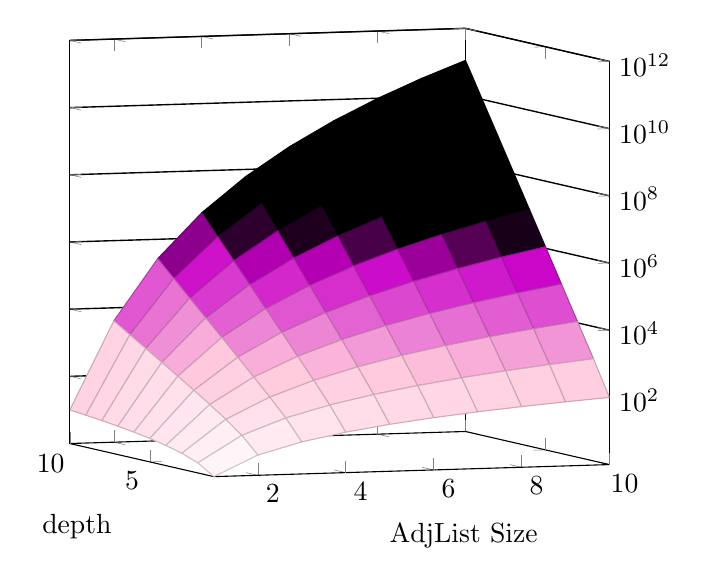
\begin{tikzpicture}
\begin{axis}[
    xlabel={AdjList Size},
    ylabel={depth},
    zmode=log,
    zmin=1e0,
    zmax=1e12,
    zticklabel pos=right,
    ztick={1e2, 1e4, 1e6, 1e8, 1e10, 1e12},
    zmajorgrids=true,
    grid style={line width=0.5pt, draw=black},
    view={-20}{5},
    % colormap name=viridis,
    % shader=interp,
    colormap={custom}{ % Define a custom colormap
        [1cm] 
        color(0cm)=(white) 
        % rgb255(1cm)=(50,255,230)
        % color(1cm)=(cyan)
        rgb255(25cm)=(255,200,220)
        rgb255(50cm)=(200,0,200)
        % color(2cm)=(violet)
        color(59cm)=(black)
        % rgb255(4cm)=(60,20,60)
        % rgb255(5cm)=(100,80,100)
        color(100cm)=(black)}
    ]
\addplot3[surf,] 
coordinates{
(1,1,1) (1,2,2) (1,3,3) (1,4,4) (1,5,5) (1,6,6) (1,7,7) (1,8,8) (1,9,9) (1,10,10) 

(2,1,4) (2,2,12) (2,3,28) (2,4,60) (2,5,124) (2,6,252) (2,7,508) (2,8,1020) (2,9,2044) (2,10,4092) 

(3,1,9) (3,2,36) (3,3,117) (3,4,360) (3,5,1089) (3,6,3276) (3,7,9837) (3,8,29520) (3,9,88569) (3,10,265716) 

(4,1,16) (4,2,80) (4,3,336) (4,4,1360) (4,5,5456) (4,6,21840) (4,7,87376) (4,8,349520) (4,9,1398096) (4,10,5592400) 

(5,1,25) (5,2,150) (5,3,775) (5,4,3900) (5,5,19525) (5,6,97650) (5,7,488275) (5,8,2441400) (5,9,12207025) (5,10,61035150) 

(6,1,36) (6,2,252) (6,3,1548) (6,4,9324) (6,5,55980) (6,6,335916) (6,7,2015532) (6,8,12093228) (6,9,72559404) (6,10,435356460) 

(7,1,49) (7,2,392) (7,3,2793) (7,4,19600) (7,5,137249) (7,6,960792) (7,7,6725593) (7,8,47079200) (7,9,329554449) (7,10,2306881192) 

(8,1,64) (8,2,576) (8,3,4672) (8,4,37440) (8,5,299584) (8,6,2396736) (8,7,19173952) (8,8,153391680) (8,9,1227133504) (8,10,9817068096) 

(9,1,81) (9,2,810) (9,3,7371) (9,4,66420) (9,5,597861) (9,6,5380830) (9,7,48427551) (9,8,435848040) (9,9,3922632441) (9,10,35303692050) 

(10,1,100) (10,2,1100) (10,3,11100) (10,4,111100) (10,5,1111100) (10,6,11111100) (10,7,111111100) (10,8,1111111100) (10,9,11111111100) (10,10,111111111100)
};
\end{axis}
\end{tikzpicture}
\caption{Number of query atoms in relation to \texttt{AdjList} size and navigation depth}
    \label{fig:navcount}
    \Description[AST]{}
\end{figure}


The complete navigation model has twice as many constraints $2f(N,d)$, as we need both an element and some pointer arithmetic for each intermediate variable. 
Our implementation of the pointer arithmetic implies an additional intermediate variable, giving a total of $2f(N,d)$ intermediate variables.
% To quote \cite{jackson_alcoa_2000} the models resulting from the relational logic are \emph{huge}.

The total number of propagations required to find all counter proofs, or validate a model also aligns with the number of constraints found here $2f(N,d)$, validation would correspond to all the problem variables having only one possible value. 
While it is a large number it's still fast to run all these propagators once, and running out of memory space for the model became a more limiting factor than time in our tests.

Going beyond validation, and searching for a model fix, or completing a model such as in our use-case, means increasing the domains of the problem variables and by consequence the intermediate variables, and in the case of model completion having the full range of possibilities for all these variables.

\subsubsection{Subset Sum Problem}\footnote{\url{https://github.com/ArtemisLemon/navCSP_SubsetSum}}
by applying the following constraints to the query from a single object (among up to 120), we can model a variation on the subset sum problem:
$$\texttt{query->sum(attribute) = Target}$$
$$\texttt{and query->isUnique(attribute)}$$
Where \texttt{self.attribute} of an object is a constant integer attribute between 10 and 29. 
All of them together forming a multiset, from which we'll find a subset with the right sum.
Initial testing with this problem gives fast non-trivial solutions, up to a few minutes, for queries with up to around $10^4$ intermediate variables.
When no subset sums equal the target, such as finding a subset summing to 1, or when solving for trivial targets such as 0, the process takes less than a few minutes up to $10^6$ intermediate variables.
% If we were to attempt model repair, we could slightly increase the domain around the disproven values, and search for models in that space, which would be much smaller than in this context.
% Taking in total less than minute for up to $10^5$ intermediate variables.
Bigger problems reached our memory limit.
% Another notable observation, is building the Choco CSP often takes longer than disproving this case. 
% \ytodo{apply to all objects?}
These results color \autoref{fig:navcount}, the lightest area being quickly solvable, the darker area being quickly verifiable and the black area being too big to model.

% The evaluation instance will all follow the same pattern.
% The multisets will be the first M elements of a repeating sequences of $[10..30[$.
% The target sums will be 10 as it will appear in all the multisets, the max subset sum $S=\frac{M}{2}*(10+(10+M-1))$ of a multiset.
% In cases where there is a solution path, those values will be bold?

% To get solutions, we search in the problem variables, here those representing the references, and the variable to which the top most constraint is applied. 

\subsection{RMS use-case} 
In our running example, our instance will have 4 stages (S) and 43 task (T), directly taken from \cite{Wang2012-srms}. We infer 24 machines (M) from their constraint model.
In our annotation of \texttt{machines} we will choose 24 as the maximum cardinality of the reference, and thus have 24 pointer variables in the associated \texttt{AdjList}.
Notice that the combinatorial complexity of the problem is quite challenging, since there are around $2.10^{40}$ possible graphs satisfying these assumptions. Generating all graphs and checking the OCL constraints would be unfeasible.  
The full code for this problem instance is available online.\footnote{\url{https://github.com/ArtemisLemon/navCSP_RMSTaskConstraints}}
% Tasks are linked to at most one stage, so the reference is given an AdjLink variable with a single pointer variable.
% The reference from stage to machine is unbounded in the metamodel of \autoref{fig:uc_uml}, an upper bound will there for have to be defined in the annotation.
% In the original use case, the space constraint bounded this number to 6 for all stages, which will be the value used for times.
% In other measurements, this value will be a variable $N$.

% This work is also ... by previous work on ATLc, which provides an solving for OCL constraints on attributes. 
% In a way, providing human-in-the-loop optimisation, and domain space exploration.
% This requires fast solving.

\begin{table}[ht]
\begin{tabular}{|c|r|r|r|r|}
\hline
\multicolumn{1}{|l|}{\textbf{var()}} & \multicolumn{1}{l|}{\textbf{variables}} & \multicolumn{1}{l|}{\textbf{domain}} & \multicolumn{1}{l|}{\textbf{constraints}} & \multicolumn{1}{l|}{\textbf{time}} \\ \hline
\multirow{2}{*}{stage}                                                      & 43 & S & \multirow{2}{*}{(43)} & \multirow{2}{*}{0.1s}              \\ \cline{2-3}
                                                                            & 0 & M & & \\ \hline
\multirow{2}{*}{machines}                                                   & 0 & S & \multirow{2}{*}{(96)} & \multirow{2}{*}{0.1s}              \\ \cline{2-3}
                                                                            & 96 & M & &                                    \\ \hline
\multirow{2}{*}{\begin{tabular}[c]{@{}c@{}}stage\\ machines\end{tabular}}   & 43 & S & \multirow{2}{*}{2064 (+1032)} & \multirow{2}{*}{0.3s}              \\ \cline{2-3}
                                                                            & 96+1032 & M &                                           &                                    \\ \hline
\end{tabular}
\caption{Size and resolution times of the use-case CSPs}
\label{tab:rms_results}
\end{table}

In \autoref{tab:rms_results} we find the metrics for the three RMS scenarios.
Additionally to the same characteristic constraint, we also enforce the precedence constraint in the scenarios where the reference \texttt{Task.stage} is annotated.    
The first column identifies the annotations, and the scenarii.
The second column gives the variable counts for each domain.
The variable count includes all variables (problem and intermediate) involved in the expression.
While the intermediate variable are unique to the model of this expression, the problem variables (tied to the instance objects) are shared by any other expression.
Domains, informed by the third column, are identified by their upper bound, as the lower bound generally 0 for pointer variables.
For the last row, we have both 96 problem variables of domain M, and because of the navigation from the 43 problem variables of domain S, each requiring their own copies of the variables of domain M, there are 1032 (43*N) intermediate variables.

In the constraints column, we count constraints of the OCL CSP, mainly element constraints and pointer arithmetic.
In between brackets is the counter of $member$ constraints.
As $member$ only propagates once, by default our solver doesn't include them in the constraint count.
As it is the only constraint in two of these cases, we have included them.

Finally for times, we can see this problem is trivial for the solver.
Most of the time taken is to build the model.

\section{Limitations and Future Work}
\label{sec:disc}
% \ynote{
% \subsection{Annotated OCL as a Language for Solver Collaboration}
% \texttt{stage.var('machines', 'Choco').var('powerSetting', 'Cassowary')}
% }{}

% \subsection{Alternative Annotations}
% Here we propose annotations in the OCL constraints as it suits our use.
% It also allows us to only model the relevant end of an association.
% For example we model the references from \texttt{Task} to \texttt{Stage}, but didn't need to model the opposite, and the coherence between both ends.

% These annotations could be placed on the class diagram or similar formalism (ECore and xcore for example, or even z-notion), or as a header to the OCL declaration, to better suit modeling needs.
% All of these choices would result in the same annotations of the OCL ASTs.


\noindent \textbf{Alternative CP Models.}
Here we present a navigation model based on pointers, modeled by lists of integer variables.
In OCL the result of accessing a reference and navigation is of type collection,
and there are 4 concrete collection types, at the crossroads of two qualities: orderedness and uniqness.
This pointer variable model provides a representation for ordered collections with non-unique elements, or the OCL collection type \texttt{Sequence}.
Applying \texttt{AllDifferent} can model the collection type \texttt{OrderedSet}.
The other OCL collection types, namely \texttt{Set} and \texttt{Bag}, can be modeled differently and more efficiently.
Notably references and navigation as \texttt{Set} can make use of \emph{set variables} which can answer the question \emph{which objects are connected to the given object?}, the global constraint $union(y : set, vars : set[], z : set)$, mirroring the element constraint, and trivially providing efficient variable navigation.

Navigation in OCL often resolves to Sequences of pointers, hence a requirement to model them to maximize OCL coverage.
But if modeling with constraint enforcing in mind, it is interesting to ask if orderedness is important to your navigations, as it is a costly quality.
Choosing between these encodings for references could be informed by the annotations. 

% \ytodo{recently written, Theo is doing a first pass}
\noindent \textbf{Further Evaluation.}
Initial evaluations unsurprisingly revealed navigation is a complex issue, however it also revealed its complexity is complex to measure.
We give the size of the navCSP in terms of intermediate variables and constraints, but the domain size of the variables, the number of objects and types, are among the another variables.
And while we give some aspect of the size, it doesn't tell the whole story of how hard a problem is to solve.
Models with low \texttt{AdjList} size and deep navigation are very difficult problems, even if the overall model is small.
While models with larger \texttt{AdjList} variables and shallow navigation depths produce large problems that can sometimes be solved faster.
Graph density is also an interesting dimension. 
Additionally the complete evaluation for this method requires comparisons to Alloy \cite{Jackson2002-alloy} as it applies SAT techniques \cite{Torlak2007-kodkod} for model finding.

\noindent \textbf{Automation of the Refactoring.} 
As hinted as in \autoref{ssec:refactor}, some OCL refactoring seems to be systematically applicable.
However it does require more computation ahead of building the CSP.
This method needs to be formalised and the pre-computation tested for efficiency gains.
For our use case, the pre-computation around \texttt{forall} was trivial, but allowed for instant solving times.
The general case however allows for much more complex pre-computation.

\noindent \textbf{Translating Full OCL.}
In this paper, we focus on the translation for the OCL \texttt{NavigationOrAttributeCallExp} node. 
We also hint at a translation of \texttt{includesAll} using the member constraint, but all collection operations can be similarly modeled in CP, with varying efficiency.
Finding the models using global constraints for OCL words isn't trivial, and finding efficient ones may require testing and even the development of new propagation algorithms.
Having a translation scheme for each OCL word, will allow us to implement a compiler, and integrate it into a model transformation framework such as ATLc \cite{Le_Calvar2021-solvers}, giving us a framework to implement model repair and domain space exploration.

\noindent \textbf{Application to Design Space Exploration and Integration with ATLc.}
ATLc is an extension to the ATL transformation language, based on OCL, which couples constraint solvers \cite{Le_Calvar2021-solvers} with incremental model transformations \cite{Le_Calvar2019-atol}. 
The greater objective of this work is to add to the ATLc compiler, and use it's GUI framework to generate interfaces, allowing users to interact with the search for solutions to structural constraints, in a form of human-in-the-loop solving. 
% This would allow for a form of human-in-the-loop solving and optimisation.











\section{Related Work} \label{sec:related}

% \begin{outline}
%     \1 ATLc
%         \2 ATL
%     \1 QVTc
%     \1 Viatra
%     \1 New Pb 4 CSP: OO modeling 
%         \2 
% \end{outline}

The most similar work to our overall objective is by Le Calvar et al. \cite{Le_Calvar2021-solvers}, which provides a tool for domain space exploration by means of model transformations coupled with CP solvers.
This work provides the compilation of arithmetic OCL constraints on attributes to a variety of constraint solvers.
This work also provides a framework for modeling CSPs on Java GUIs and also discusses weakening constraints, and solver collaboration.
However this compiler doesn't provide the compilation of structural constraints; they provide \emph{variable property access} but not \emph{variable navigation}.
Because of this they don't require an annotation system, as they can assume that the top level of the query is the variable.
% And our overall objective would be to add this to their compiler.
%Among the following, are related works identified by this previous work. 
% This previous work points to related works, among the following.

% The work also cites \cite{petter_solving_2009} as their most relevant work, along with a number of others.
% They propose a solution allowing for arithmetic constraints on numeric attributes of target models of QVT transformations.
% Similarly, it extends the semantics of the OCL in a transformation language, but focuses on cases which result in variables representing attributes.
% A notable difference is this fifort translates the whole transformation to an Eclipse prolog specification.

% This is similar to the early proposition for Design (model) Space Exploration \cite{schatz_design-space_2010}, which encodes the transformation problem in prolog, but doesn't yet use a Transformation Language or OCL to describe the problem.

% ,jackson_alcoa_2000
Alloy \cite{Jackson2002-alloy} also provides a modeling language similar to UML and OCL, based on the Z specification language with it's own query language.
Allowing the declaration of problems over it's OCL-inspired query language makes it particularly relevant to what we present in this paper.
% Much like us it provides model space exploration, but again relying on prolog.
This also points at a first difference, the choice of source constraint language: Alloy provides it's own language, where we try to cover a well established standard.
To analyze models the Alloy toolkit uses KodKod \cite{Torlak2007-kodkod} to translate the problems towards SAT solvers for verification and model finding.
This is similar to our work, but we translate the problem to global constraint models.
Both SAT and CSP can similarly model the problem, but they each provide different methods to find a solution.
These different methods provide \emph{off-the-shelf} solvers such as Choco, which also provides a framework to develop propagators.  
Choosing between SAT and CSP to model and solve a problem isn't simple, but the ability to design propagators and direct search makes it an interesting avenue to pursue.
With our work, we lay the foundations to explore the alternative.
% \ytodo{Further experimentation will be interesting to compare both (does one work better for different graph densities, etc..)}

Another example, which bares strong resemblance to our work is that of \cite{Bergmann2015-viatra,Horvath2009-cspm}. Constraints on target models are encoded as patterns of elements.
This work gives rise to CSP(m) for Viatra, allowing visual pattern mappings to define transformation rules, with anti-patterns similar to constraints to enforce.
CSP(m) is a solver based on backtracking algorithms designed for this specific purpose, which also solves the whole transformation.
This differs from our solution which reuses \emph{off the shelf} tools to model the problem, and global constraints on integers which are implemented by many of these solvers.
% Solutions to the transformation respecting those patterns, are found using the backtracking algorithm behind prolog. 
Solving for the whole transformation is another significant difference, as ATLc splits the effort between tools better suited to their respective tasks. 
Alleviating the constraint solver, and leveraging the efficiency of the transformation engine \cite{Le_Calvar2019-atol}.
% This also limits the ability to perform domain space exploration, and Viatra's main application is efficient validation through transformations.
% Other effort relating constraints and transformations also tend to differ this way, creating transformation engines or solvers as opposed to re-using them.

% Beyond model space explorations there is also work bridging UML modeling and constraints, of which the OCL language is a core artifact to be verified.
% A notable example of this is EMFtoCSP \cite{cabot_umltocsp_2007,gonzalez_emftocsp_2012}, which similarly uses Eclipse Prolog, to verify models, and Viatra which also allows EMF model checking and transformation.





% This work also has similarities with the Comma CP language \cite{soto_design_2007}.
% Which provides syntax to organise variables, and constraints upon them.
% This work differs by proposing a new language to \emph{model using objects}, whereas we reuse an EMF models.
% UML also allows for queries on the model, which isn't a problem addressed in this related work.
% This, among others, attempts to answer the challenge of \emph{simplicity of use}, as defined in \cite{hutchison_constraint_2004}.
% Which specifies a "Model and Run" paradigm for constraint modeling, and calls for it's implementation.
% This paper starts to answer two points, \emph{file standardisation}, which would be answered by UML standards (XMI), and \emph{a library of CP algorithms which can take such models and solve them}, which we provide with model transformations using an OCL to CSP compiler.

% \mtodo{ok but you must explain where the current work is better than all the others!}

\section{Conclusion}\label{sec:qed} 
% \ytodo{1 page with \autoref{sec:related}}

%\begin{outline}
% \1 Having solved navigation
%     \2 finishing implementation
%     \2 for link variables, and occurrence variables
%     \2 we can now translate all operators for references
%     \2 we can now tackle collections in general
%     \2 solve navigation for occurrence with out adding link symmetries
% \1 Reconfiguration Loop
%     \2 Loop
%         \3 find solutions based on current data
%         \3 user makes changes and chooses what part of the solution to keep, which is added to the data
%         \3 repeat
%     \2 requirement: (G)UI
%     \2 RMS reconfiguration App
% \1 Evaluation against optimal CSPs
%     \2 for ocl constraint (regardless of compilation)
%     \2 for a problem (no uml)
% % \1 Improving Solvers
% %     \2 improve current global propagators
% %     \2 identify new globals and propagators
%\end{outline}

% Stood on the shoulders of giants (or at least \emph{very tall people from afar}) and got high.
% It's a bit of a balancing act.

We have shown how to model the core of OCL queries and navigations using CP, laying the foundation of modeling OCL with global constraints. We did so using models encoding orderedness and non-uniqueness of OCL Sequences, the most complex version of the problem.
The models are also designed to be assembled by an OCL compiler.
To identify variables during compilation and guide CP modeling, we have proposed the \texttt{var()} operator as an annotation of the OCL constraint model.
We have also raised the question of how to better model OCL with enforcing in mind, which hints at a systematic method applied during static analysis.
We have also outlined other branches of future work, such as: further modeling OCL using global constraints, implementation atop of ATLc, and evaluation and comparison with other methods.
